\documentclass[border=10pt,11pt]{standalone}
\usepackage[T1]{fontenc}
\usepackage{lmodern}
\usepackage{amsmath, amssymb}
\usepackage{xcolor}
\definecolor{NavyAccent}{HTML}{1A3A5C}
\definecolor{InkColor}{HTML}{1F2937}
\definecolor{SubInk}{HTML}{4B5563}
\definecolor{CardBG}{HTML}{F4F6F8}
\definecolor{AccentBlue}{HTML}{2E86DE}
\definecolor{GoodGreen}{HTML}{1B8E4F}
\definecolor{BadRed}{HTML}{C0392B}
\definecolor{WarnAmber}{HTML}{C97B12}
\usepackage{tikz}
\usetikzlibrary{positioning, arrows.meta, shapes.geometric, shadows, fit, backgrounds, calc}

\newcommand{\nz}{n_{z}}

\begin{document}
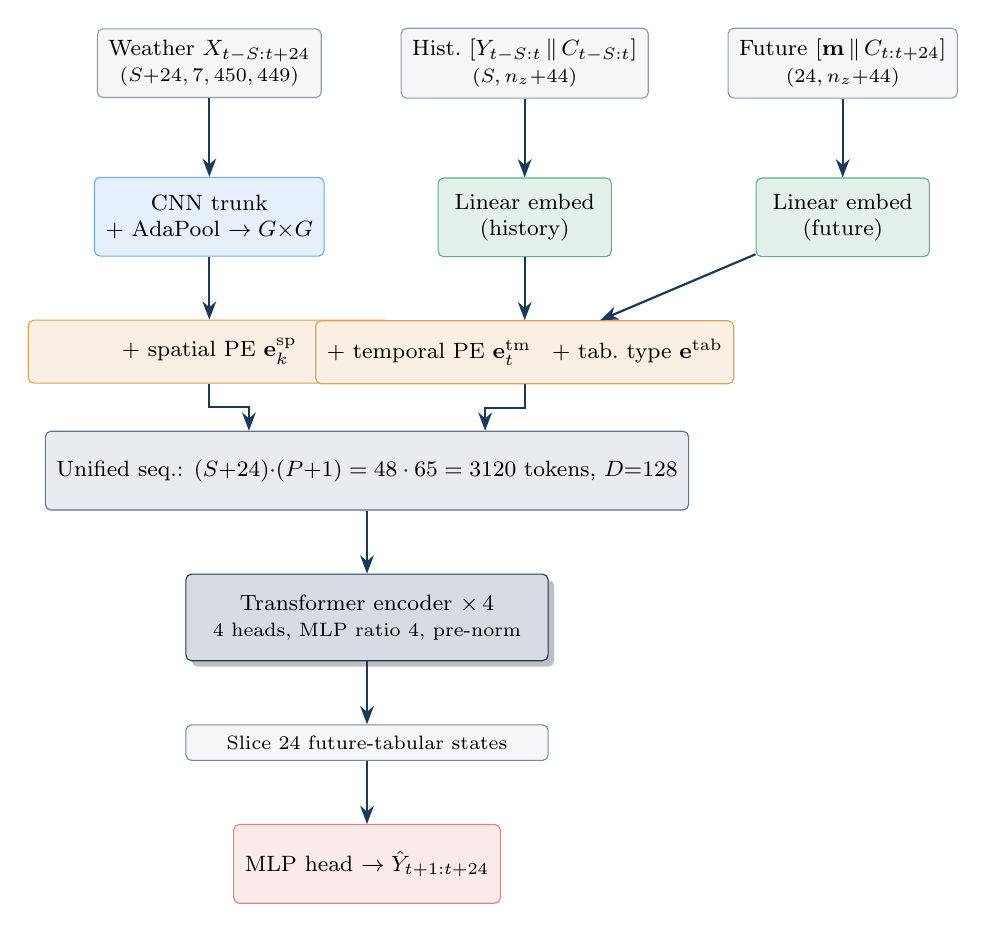
\begin{tikzpicture}[
    >=Stealth, node distance=8mm and 10mm,
    box/.style={draw, rounded corners=2pt, align=center, font=\footnotesize, inner sep=4pt},
    inputbox/.style={box, fill=CardBG, draw=NavyAccent!50, minimum height=8mm, minimum width=22mm},
    cnnbox/.style={box, fill=AccentBlue!12, draw=AccentBlue!70, minimum height=10mm, minimum width=22mm},
    tabbox/.style={box, fill=GoodGreen!12, draw=GoodGreen!70, minimum height=10mm, minimum width=22mm},
    posbox/.style={box, fill=WarnAmber!12, draw=WarnAmber!70, minimum height=8mm, minimum width=46mm},
    seqbox/.style={box, fill=NavyAccent!10, draw=NavyAccent!70, minimum height=10mm, minimum width=64mm},
    txbox/.style={box, fill=NavyAccent!18, draw=NavyAccent, minimum height=11mm, minimum width=46mm, drop shadow},
    outbox/.style={box, fill=BadRed!10, draw=BadRed!60, minimum height=10mm, minimum width=30mm},
    arr/.style={->, thick, NavyAccent},
    lab/.style={font=\scriptsize\itshape, color=SubInk}
]
\node[inputbox] (xw) {Weather $X_{t-S:t+24}$\\\scriptsize $(S{+}24,7,450,449)$};
\node[inputbox, right=of xw] (xt) {Hist.\ $[Y_{t-S:t}\,\Vert\,C_{t-S:t}]$\\\scriptsize $(S, \nz{+}44)$};
\node[inputbox, right=of xt] (xf) {Future $[\mathbf{m}\,\Vert\,C_{t:t+24}]$\\\scriptsize $(24, \nz{+}44)$};
\node[cnnbox, below=10mm of xw] (cnn) {CNN trunk\\$+$ AdaPool $\to G{\times}G$};
\node[tabbox, below=10mm of xt] (lin1) {Linear embed\\(history)};
\node[tabbox, below=10mm of xf] (lin2) {Linear embed\\(future)};
\node[posbox, below=8mm of cnn] (sp) {$+$ spatial PE $\mathbf{e}^{\mathrm{sp}}_k$};
\node[posbox, below=8mm of lin1] (tp) {$+$ temporal PE $\mathbf{e}^{\mathrm{tm}}_t$ \;\;$+$ tab.\ type $\mathbf{e}^{\mathrm{tab}}$};
\node[seqbox, below=10mm of $(sp)!0.5!(tp)$] (seq) {Unified seq.: $(S{+}24){\cdot}(P{+}1) = 48 \cdot 65 = 3120$ tokens, $D{=}128$};
\node[txbox, below=8mm of seq] (tx) {Transformer encoder $\times\,4$\\\scriptsize 4 heads, MLP ratio 4, pre-norm};
\node[box, below=8mm of tx, fill=CardBG, draw=NavyAccent!60, minimum width=46mm, font=\scriptsize] (slice) {Slice 24 future-tabular states};
\node[outbox, below=8mm of slice] (head) {MLP head $\to\hat Y_{t+1:t+24}$};
\draw[arr] (xw) -- (cnn);
\draw[arr] (xt) -- (lin1);
\draw[arr] (xf) -- (lin2);
\draw[arr] (cnn) -- (sp);
\draw[arr] (lin1) -- (tp);
\draw[arr] (lin2) -- (tp);
\draw[arr] (sp.south) -- ++(0,-3mm) -| ([xshift=-15mm]seq.north);
\draw[arr] (tp.south) -- ++(0,-3mm) -| ([xshift=15mm]seq.north);
\draw[arr] (seq) -- (tx);
\draw[arr] (tx) -- (slice);
\draw[arr] (slice) -- (head);
\end{tikzpicture}
\end{document}
